\documentclass[twoside]{book}

% Packages required by doxygen
\usepackage{fixltx2e}
\usepackage{calc}
\usepackage{doxygen}
\usepackage[export]{adjustbox} % also loads graphicx
\usepackage{graphicx}
\usepackage[utf8]{inputenc}
\usepackage{makeidx}
\usepackage{multicol}
\usepackage{multirow}
\PassOptionsToPackage{warn}{textcomp}
\usepackage{textcomp}
\usepackage[nointegrals]{wasysym}
\usepackage[table]{xcolor}

% NLS support packages
Portuguese
% Font selection
\usepackage[T1]{fontenc}
\usepackage[scaled=.90]{helvet}
\usepackage{courier}
\usepackage{amssymb}
\usepackage{sectsty}
\renewcommand{\familydefault}{\sfdefault}
\allsectionsfont{%
  \fontseries{bc}\selectfont%
  \color{darkgray}%
}
\renewcommand{\DoxyLabelFont}{%
  \fontseries{bc}\selectfont%
  \color{darkgray}%
}
\newcommand{\+}{\discretionary{\mbox{\scriptsize$\hookleftarrow$}}{}{}}

% Page & text layout
\usepackage{geometry}
\geometry{%
  a4paper,%
  top=2.5cm,%
  bottom=2.5cm,%
  left=2.5cm,%
  right=2.5cm%
}
\tolerance=750
\hfuzz=15pt
\hbadness=750
\setlength{\emergencystretch}{15pt}
\setlength{\parindent}{0cm}
\setlength{\parskip}{0.2cm}
\makeatletter
\renewcommand{\paragraph}{%
  \@startsection{paragraph}{4}{0ex}{-1.0ex}{1.0ex}{%
    \normalfont\normalsize\bfseries\SS@parafont%
  }%
}
\renewcommand{\subparagraph}{%
  \@startsection{subparagraph}{5}{0ex}{-1.0ex}{1.0ex}{%
    \normalfont\normalsize\bfseries\SS@subparafont%
  }%
}
\makeatother

% Headers & footers
\usepackage{fancyhdr}
\pagestyle{fancyplain}
\fancyhead[LE]{\fancyplain{}{\bfseries\thepage}}
\fancyhead[CE]{\fancyplain{}{}}
\fancyhead[RE]{\fancyplain{}{\bfseries\leftmark}}
\fancyhead[LO]{\fancyplain{}{\bfseries\rightmark}}
\fancyhead[CO]{\fancyplain{}{}}
\fancyhead[RO]{\fancyplain{}{\bfseries\thepage}}
\fancyfoot[LE]{\fancyplain{}{}}
\fancyfoot[CE]{\fancyplain{}{}}
\fancyfoot[RE]{\fancyplain{}{\bfseries\scriptsize Gerado em Domingo, 8 de Novembro de 2015 15\+:27\+:18 para Transportex 1.\+0.\+0 por Doxygen }}
\fancyfoot[LO]{\fancyplain{}{\bfseries\scriptsize Gerado em Domingo, 8 de Novembro de 2015 15\+:27\+:18 para Transportex 1.\+0.\+0 por Doxygen }}
\fancyfoot[CO]{\fancyplain{}{}}
\fancyfoot[RO]{\fancyplain{}{}}
\renewcommand{\footrulewidth}{0.4pt}
\renewcommand{\chaptermark}[1]{%
  \markboth{#1}{}%
}
\renewcommand{\sectionmark}[1]{%
  \markright{\thesection\ #1}%
}

% Indices & bibliography
\usepackage{natbib}
\usepackage[titles]{tocloft}
\setcounter{tocdepth}{3}
\setcounter{secnumdepth}{5}
\makeindex

% Hyperlinks (required, but should be loaded last)
\usepackage{ifpdf}
\ifpdf
  \usepackage[pdftex,pagebackref=true]{hyperref}
\else
  \usepackage[ps2pdf,pagebackref=true]{hyperref}
\fi
\hypersetup{%
  colorlinks=true,%
  linkcolor=blue,%
  citecolor=blue,%
  unicode%
}

% Custom commands
\newcommand{\clearemptydoublepage}{%
  \newpage{\pagestyle{empty}\cleardoublepage}%
}


%===== C O N T E N T S =====

\begin{document}

% Titlepage & ToC
\hypersetup{pageanchor=false,
             bookmarks=true,
             bookmarksnumbered=true,
             pdfencoding=unicode
            }
\pagenumbering{roman}
\begin{titlepage}
\vspace*{7cm}
\begin{center}%
{\Large Transportex 1.0.0 }\\
\vspace*{1cm}
{\large Gerado por Doxygen 1.8.10}\\
\vspace*{0.5cm}
{\small Domingo, 8 de Novembro de 2015 15:27:18}\\
\end{center}
\end{titlepage}
\clearemptydoublepage
\tableofcontents
\clearemptydoublepage
\pagenumbering{arabic}
\hypersetup{pageanchor=true}

%--- Begin generated contents ---
\chapter{Índice dos componentes}
\section{Lista de componentes}
Lista de classes, estruturas, uniões e interfaces com uma breve descrição\+:\begin{DoxyCompactList}
\item\contentsline{section}{\hyperlink{class_camiao}{Camiao} }{\pageref{class_camiao}}{}
\item\contentsline{section}{\hyperlink{class_camiao_inexistente}{Camiao\+Inexistente} }{\pageref{class_camiao_inexistente}}{}
\item\contentsline{section}{\hyperlink{class_cliente}{Cliente} }{\pageref{class_cliente}}{}
\item\contentsline{section}{\hyperlink{class_cliente_inexistente}{Cliente\+Inexistente} }{\pageref{class_cliente_inexistente}}{}
\item\contentsline{section}{\hyperlink{class_empresa}{Empresa} }{\pageref{class_empresa}}{}
\item\contentsline{section}{\hyperlink{class_frota}{Frota} }{\pageref{class_frota}}{}
\item\contentsline{section}{\hyperlink{class_servico}{Servico} }{\pageref{class_servico}}{}
\item\contentsline{section}{\hyperlink{class_servico_inexistente}{Servico\+Inexistente} }{\pageref{class_servico_inexistente}}{}
\end{DoxyCompactList}

\chapter{Documentação da classe}
\hypertarget{class_camiao}{}\section{Referência à classe Camiao}
\label{class_camiao}\index{Camiao@{Camiao}}


Diagrama de colaboração para Camiao\+:
\nopagebreak
\begin{figure}[H]
\begin{center}
\leavevmode
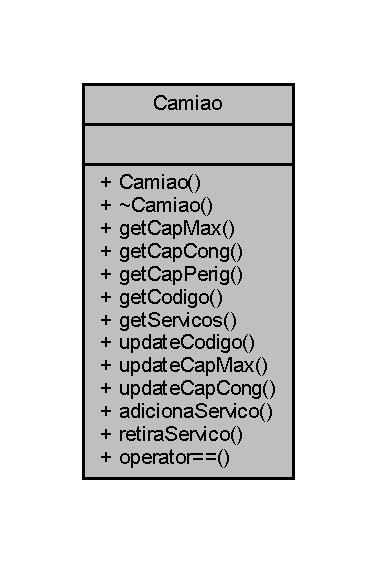
\includegraphics[width=181pt]{class_camiao__coll__graph}
\end{center}
\end{figure}
\subsection*{Membros públicos}
\begin{DoxyCompactItemize}
\item 
\hyperlink{class_camiao_a9dbe2b8fd232262b23cb7817634ec9f2}{Camiao} (int codigo, unsigned int cap\+\_\+max, bool cap\+\_\+cong, bool cap\+\_\+perig)
\begin{DoxyCompactList}\small\item\em Cria um Camião usando os parâmetros para definir as sua caracteristicas. \end{DoxyCompactList}\item 
unsigned int \hyperlink{class_camiao_a95ab6ea48022557c3ffa5ac5f5f100d7}{get\+Cap\+Max} () const 
\begin{DoxyCompactList}\small\item\em Obtém a Capacidade Máxima de um Camião. \end{DoxyCompactList}\item 
bool \hyperlink{class_camiao_add0d42a0b4a15e9cd3f4b0626567bddf}{get\+Cap\+Cong} () const 
\begin{DoxyCompactList}\small\item\em Verifica se um Camião tem ou não capacidade de congelação. \end{DoxyCompactList}\item 
bool \hyperlink{class_camiao_ad779b545bf87564fb761a89cc0fdb5b2}{get\+Cap\+Perig} () const 
\begin{DoxyCompactList}\small\item\em Verifica se um Camião tem ou não capacidade de transportar cargas perigosas. \end{DoxyCompactList}\item 
int \hyperlink{class_camiao_ad193383e9f205676df51070eea748bb1}{get\+Codigo} () const 
\begin{DoxyCompactList}\small\item\em Obtém o Código identificador de um Camião. \end{DoxyCompactList}\item 
vector$<$ \hyperlink{class_servico}{Servico} $\ast$ $>$ \hyperlink{class_camiao_aa76342c254c9e9b9873d12b2280f5260}{get\+Servicos} () const 
\begin{DoxyCompactList}\small\item\em Obtém os serviços para os quais um camião está a ser usado. \end{DoxyCompactList}\item 
void \hyperlink{class_camiao_a4f988acfcd16392ca0b104eae046fcc3}{update\+Codigo} (int codigo)
\begin{DoxyCompactList}\small\item\em Altera, se necessário, o código de um Camião. \end{DoxyCompactList}\item 
void \hyperlink{class_camiao_a1969f708e4055e48b27b0f727a985fb4}{update\+Cap\+Max} (unsigned int cap\+\_\+max)
\begin{DoxyCompactList}\small\item\em Altera, se necessário, a capacidade máxima de um Camião. \end{DoxyCompactList}\item 
void \hyperlink{class_camiao_a4bc98b0b67a9189f0f01ef1cbb06db23}{update\+Cap\+Cong} (bool cap\+\_\+cong)
\begin{DoxyCompactList}\small\item\em Altera, se necessário, o valor lógico da capacidade de congelação de um camião. \end{DoxyCompactList}\item 
void \hyperlink{class_camiao_afba93eb174b4708bd6a060193c116055}{adiciona\+Servico} (\hyperlink{class_servico}{Servico} $\ast$s1)
\begin{DoxyCompactList}\small\item\em Adiciona um serviço que utiliza o camião. \end{DoxyCompactList}\item 
void \hyperlink{class_camiao_a98fc9d0557379100c5c8483347aef88b}{retira\+Servico} (\hyperlink{class_servico}{Servico} $\ast$s1)
\begin{DoxyCompactList}\small\item\em Retira um serviço que utiliza o camião. \end{DoxyCompactList}\item 
bool \hyperlink{class_camiao_a2e09163befe964a586485ef4e3b180bd}{operator==} (const \hyperlink{class_camiao}{Camiao} \&c1)
\begin{DoxyCompactList}\small\item\em Operador utilizado para verificar se dois camiões são iguais. \end{DoxyCompactList}\end{DoxyCompactItemize}


\subsection{Documentação dos Construtores \& Destrutor}
\hypertarget{class_camiao_a9dbe2b8fd232262b23cb7817634ec9f2}{}\index{Camiao@{Camiao}!Camiao@{Camiao}}
\index{Camiao@{Camiao}!Camiao@{Camiao}}
\subsubsection[{Camiao(int codigo, unsigned int cap\+\_\+max, bool cap\+\_\+cong, bool cap\+\_\+perig)}]{\setlength{\rightskip}{0pt plus 5cm}Camiao\+::\+Camiao (
\begin{DoxyParamCaption}
\item[{int}]{codigo, }
\item[{unsigned int}]{cap\+\_\+max, }
\item[{bool}]{cap\+\_\+cong, }
\item[{bool}]{cap\+\_\+perig}
\end{DoxyParamCaption}
)}\label{class_camiao_a9dbe2b8fd232262b23cb7817634ec9f2}


Cria um Camião usando os parâmetros para definir as sua caracteristicas. 


\begin{DoxyParams}{Parâmetros}
{\em codigo} & Codigo identificador do Camião \\
\hline
{\em cap\+\_\+max} & Capacidade Máxima do Camião \\
\hline
{\em cap\+\_\+cong} & Valor Lógico da Capacidade de Congelação do Camião \\
\hline
{\em cap\+\_\+perig} & Valor Lógico da Capacidade de Transporte de Cargas Perigosas do Camião \\
\hline
{\em taxa} & Custo da utilização do camião por cada quilómetro percorrido (€/km) \\
\hline
\end{DoxyParams}
\begin{DoxyReturn}{Retorna}
Esta função não possui retorno 
\end{DoxyReturn}


\subsection{Documentação dos métodos}
\hypertarget{class_camiao_afba93eb174b4708bd6a060193c116055}{}\index{Camiao@{Camiao}!adiciona\+Servico@{adiciona\+Servico}}
\index{adiciona\+Servico@{adiciona\+Servico}!Camiao@{Camiao}}
\subsubsection[{adiciona\+Servico(\+Servico $\ast$s1)}]{\setlength{\rightskip}{0pt plus 5cm}void Camiao\+::adiciona\+Servico (
\begin{DoxyParamCaption}
\item[{{\bf Servico} $\ast$}]{s1}
\end{DoxyParamCaption}
)}\label{class_camiao_afba93eb174b4708bd6a060193c116055}


Adiciona um serviço que utiliza o camião. 


\begin{DoxyParams}{Parâmetros}
{\em $\ast$s1} & Apontador para o serviço que usa o camião \\
\hline
\end{DoxyParams}
\begin{DoxyReturn}{Retorna}
Esta função não poussui retorno 
\end{DoxyReturn}
\hypertarget{class_camiao_add0d42a0b4a15e9cd3f4b0626567bddf}{}\index{Camiao@{Camiao}!get\+Cap\+Cong@{get\+Cap\+Cong}}
\index{get\+Cap\+Cong@{get\+Cap\+Cong}!Camiao@{Camiao}}
\subsubsection[{get\+Cap\+Cong() const }]{\setlength{\rightskip}{0pt plus 5cm}bool Camiao\+::get\+Cap\+Cong (
\begin{DoxyParamCaption}
{}
\end{DoxyParamCaption}
) const}\label{class_camiao_add0d42a0b4a15e9cd3f4b0626567bddf}


Verifica se um Camião tem ou não capacidade de congelação. 

\begin{DoxyReturn}{Retorna}
Retorna o valor lógico da capacidade de congelação 
\end{DoxyReturn}
\hypertarget{class_camiao_a95ab6ea48022557c3ffa5ac5f5f100d7}{}\index{Camiao@{Camiao}!get\+Cap\+Max@{get\+Cap\+Max}}
\index{get\+Cap\+Max@{get\+Cap\+Max}!Camiao@{Camiao}}
\subsubsection[{get\+Cap\+Max() const }]{\setlength{\rightskip}{0pt plus 5cm}unsigned int Camiao\+::get\+Cap\+Max (
\begin{DoxyParamCaption}
{}
\end{DoxyParamCaption}
) const}\label{class_camiao_a95ab6ea48022557c3ffa5ac5f5f100d7}


Obtém a Capacidade Máxima de um Camião. 

\begin{DoxyReturn}{Retorna}
Retorna a Capacidade Máxima de um Camião 
\end{DoxyReturn}
\hypertarget{class_camiao_ad779b545bf87564fb761a89cc0fdb5b2}{}\index{Camiao@{Camiao}!get\+Cap\+Perig@{get\+Cap\+Perig}}
\index{get\+Cap\+Perig@{get\+Cap\+Perig}!Camiao@{Camiao}}
\subsubsection[{get\+Cap\+Perig() const }]{\setlength{\rightskip}{0pt plus 5cm}bool Camiao\+::get\+Cap\+Perig (
\begin{DoxyParamCaption}
{}
\end{DoxyParamCaption}
) const}\label{class_camiao_ad779b545bf87564fb761a89cc0fdb5b2}


Verifica se um Camião tem ou não capacidade de transportar cargas perigosas. 

\begin{DoxyReturn}{Retorna}
Retorna o valor lógico da capacidade de transporte de cargas perigosas 
\end{DoxyReturn}
\hypertarget{class_camiao_ad193383e9f205676df51070eea748bb1}{}\index{Camiao@{Camiao}!get\+Codigo@{get\+Codigo}}
\index{get\+Codigo@{get\+Codigo}!Camiao@{Camiao}}
\subsubsection[{get\+Codigo() const }]{\setlength{\rightskip}{0pt plus 5cm}int Camiao\+::get\+Codigo (
\begin{DoxyParamCaption}
{}
\end{DoxyParamCaption}
) const}\label{class_camiao_ad193383e9f205676df51070eea748bb1}


Obtém o Código identificador de um Camião. 

\begin{DoxyReturn}{Retorna}
Retorna o Código de um Camião 
\end{DoxyReturn}
\hypertarget{class_camiao_aa76342c254c9e9b9873d12b2280f5260}{}\index{Camiao@{Camiao}!get\+Servicos@{get\+Servicos}}
\index{get\+Servicos@{get\+Servicos}!Camiao@{Camiao}}
\subsubsection[{get\+Servicos() const }]{\setlength{\rightskip}{0pt plus 5cm}vector$<$ {\bf Servico} $\ast$ $>$ Camiao\+::get\+Servicos (
\begin{DoxyParamCaption}
{}
\end{DoxyParamCaption}
) const}\label{class_camiao_aa76342c254c9e9b9873d12b2280f5260}


Obtém os serviços para os quais um camião está a ser usado. 

\begin{DoxyReturn}{Retorna}
Retorna um vetor com esses serviços 
\end{DoxyReturn}
\hypertarget{class_camiao_a2e09163befe964a586485ef4e3b180bd}{}\index{Camiao@{Camiao}!operator==@{operator==}}
\index{operator==@{operator==}!Camiao@{Camiao}}
\subsubsection[{operator==(const Camiao \&c1)}]{\setlength{\rightskip}{0pt plus 5cm}bool Camiao\+::operator== (
\begin{DoxyParamCaption}
\item[{const {\bf Camiao} \&}]{c1}
\end{DoxyParamCaption}
)}\label{class_camiao_a2e09163befe964a586485ef4e3b180bd}


Operador utilizado para verificar se dois camiões são iguais. 


\begin{DoxyParams}{Parâmetros}
{\em c1} & Um dos camiões a comparar \\
\hline
\end{DoxyParams}
\begin{DoxyReturn}{Retorna}
Retorna true se os camiões forem iguais e false se não forem 
\end{DoxyReturn}
\hypertarget{class_camiao_a98fc9d0557379100c5c8483347aef88b}{}\index{Camiao@{Camiao}!retira\+Servico@{retira\+Servico}}
\index{retira\+Servico@{retira\+Servico}!Camiao@{Camiao}}
\subsubsection[{retira\+Servico(\+Servico $\ast$s1)}]{\setlength{\rightskip}{0pt plus 5cm}void Camiao\+::retira\+Servico (
\begin{DoxyParamCaption}
\item[{{\bf Servico} $\ast$}]{s1}
\end{DoxyParamCaption}
)}\label{class_camiao_a98fc9d0557379100c5c8483347aef88b}


Retira um serviço que utiliza o camião. 


\begin{DoxyParams}{Parâmetros}
{\em $\ast$s1} & Apontador para o serviço a retirar \\
\hline
\end{DoxyParams}
\begin{DoxyReturn}{Retorna}
Esta função não poussui retorno 
\end{DoxyReturn}
\hypertarget{class_camiao_a4bc98b0b67a9189f0f01ef1cbb06db23}{}\index{Camiao@{Camiao}!update\+Cap\+Cong@{update\+Cap\+Cong}}
\index{update\+Cap\+Cong@{update\+Cap\+Cong}!Camiao@{Camiao}}
\subsubsection[{update\+Cap\+Cong(bool cap\+\_\+cong)}]{\setlength{\rightskip}{0pt plus 5cm}void Camiao\+::update\+Cap\+Cong (
\begin{DoxyParamCaption}
\item[{bool}]{cap\+\_\+cong}
\end{DoxyParamCaption}
)}\label{class_camiao_a4bc98b0b67a9189f0f01ef1cbb06db23}


Altera, se necessário, o valor lógico da capacidade de congelação de um camião. 


\begin{DoxyParams}{Parâmetros}
{\em cap\+\_\+cong} & Novo valor \\
\hline
\end{DoxyParams}
\begin{DoxyReturn}{Retorna}
Esta função não possui retorno 
\end{DoxyReturn}
\hypertarget{class_camiao_a1969f708e4055e48b27b0f727a985fb4}{}\index{Camiao@{Camiao}!update\+Cap\+Max@{update\+Cap\+Max}}
\index{update\+Cap\+Max@{update\+Cap\+Max}!Camiao@{Camiao}}
\subsubsection[{update\+Cap\+Max(unsigned int cap\+\_\+max)}]{\setlength{\rightskip}{0pt plus 5cm}void Camiao\+::update\+Cap\+Max (
\begin{DoxyParamCaption}
\item[{unsigned int}]{cap\+\_\+max}
\end{DoxyParamCaption}
)}\label{class_camiao_a1969f708e4055e48b27b0f727a985fb4}


Altera, se necessário, a capacidade máxima de um Camião. 


\begin{DoxyParams}{Parâmetros}
{\em cap\+\_\+max} & Novo valor \\
\hline
\end{DoxyParams}
\begin{DoxyReturn}{Retorna}
Esta função não possui retorno 
\end{DoxyReturn}
\hypertarget{class_camiao_a4f988acfcd16392ca0b104eae046fcc3}{}\index{Camiao@{Camiao}!update\+Codigo@{update\+Codigo}}
\index{update\+Codigo@{update\+Codigo}!Camiao@{Camiao}}
\subsubsection[{update\+Codigo(int codigo)}]{\setlength{\rightskip}{0pt plus 5cm}void Camiao\+::update\+Codigo (
\begin{DoxyParamCaption}
\item[{int}]{codigo}
\end{DoxyParamCaption}
)}\label{class_camiao_a4f988acfcd16392ca0b104eae046fcc3}


Altera, se necessário, o código de um Camião. 


\begin{DoxyParams}{Parâmetros}
{\em codigo} & Novo valor \\
\hline
\end{DoxyParams}
\begin{DoxyReturn}{Retorna}
Esta função não possui retorno 
\end{DoxyReturn}


A documentação para esta classe foi gerada a partir dos seguintes ficheiros\+:\begin{DoxyCompactItemize}
\item 
C\+:/\+Users/josea/\+Documents/\+Git\+Hub/\+A\+E\+D\+A-\/\+Part1/Camiao.\+h\item 
C\+:/\+Users/josea/\+Documents/\+Git\+Hub/\+A\+E\+D\+A-\/\+Part1/Camiao.\+cpp\end{DoxyCompactItemize}

\hypertarget{class_camiao_inexistente}{}\section{Referência à classe Camiao\+Inexistente}
\label{class_camiao_inexistente}\index{Camiao\+Inexistente@{Camiao\+Inexistente}}


Diagrama de colaboração para Camiao\+Inexistente\+:
\nopagebreak
\begin{figure}[H]
\begin{center}
\leavevmode
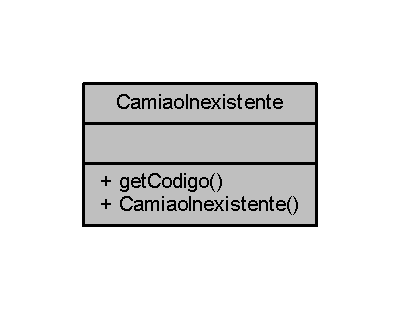
\includegraphics[width=192pt]{class_camiao_inexistente__coll__graph}
\end{center}
\end{figure}
\subsection*{Membros públicos}
\begin{DoxyCompactItemize}
\item 
\hypertarget{class_camiao_inexistente_afbb6e45281a2b470d12dc576f06a35c4}{}int {\bfseries get\+Codigo} ()\label{class_camiao_inexistente_afbb6e45281a2b470d12dc576f06a35c4}

\item 
\hypertarget{class_camiao_inexistente_ad7916f06574444a714938a4abb91c211}{}{\bfseries Camiao\+Inexistente} (int codigo)\label{class_camiao_inexistente_ad7916f06574444a714938a4abb91c211}

\end{DoxyCompactItemize}


A documentação para esta classe foi gerada a partir do seguinte ficheiro\+:\begin{DoxyCompactItemize}
\item 
C\+:/\+Users/josea/\+Documents/\+Git\+Hub/\+A\+E\+D\+A-\/\+Part1/Camiao.\+h\end{DoxyCompactItemize}

\hypertarget{class_cliente}{}\section{Referência à classe Cliente}
\label{class_cliente}\index{Cliente@{Cliente}}


Diagrama de colaboração para Cliente\+:
\nopagebreak
\begin{figure}[H]
\begin{center}
\leavevmode
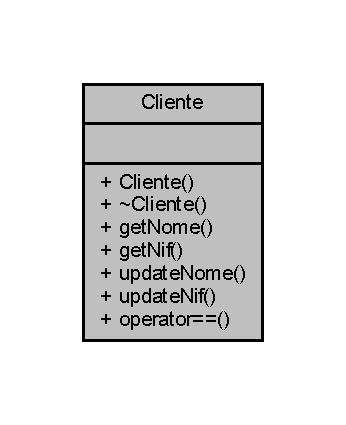
\includegraphics[width=166pt]{class_cliente__coll__graph}
\end{center}
\end{figure}
\subsection*{Membros públicos}
\begin{DoxyCompactItemize}
\item 
\hyperlink{class_cliente_a32ef83e95c16d04dd21d3063dc741b2b}{Cliente} (string nome, unsigned int nif)
\begin{DoxyCompactList}\small\item\em Cria um \hyperlink{class_cliente}{Cliente} usando os parâmetros para definir as sua caracteristicas. \end{DoxyCompactList}\item 
string \hyperlink{class_cliente_a0325de899469e2fed48ffda2b5b291cf}{get\+Nome} () const 
\begin{DoxyCompactList}\small\item\em Obtém o Nome de um \hyperlink{class_cliente}{Cliente}. \end{DoxyCompactList}\item 
unsigned int \hyperlink{class_cliente_acdfcf2501116ef255f082fa8cbcf00f2}{get\+Nif} () const 
\begin{DoxyCompactList}\small\item\em Obtém o N\+I\+F de um \hyperlink{class_cliente}{Cliente}. \end{DoxyCompactList}\item 
void \hyperlink{class_cliente_a64bdc5ca23f1d781b5bb4d9bc42f773f}{update\+Nome} (string nome)
\begin{DoxyCompactList}\small\item\em Altera, se necessário, o nome de um \hyperlink{class_cliente}{Cliente}. \end{DoxyCompactList}\item 
void \hyperlink{class_cliente_a84df96f0f9cd1aa064fc80f98dc3ccbc}{update\+Nif} (unsigned int nif)
\begin{DoxyCompactList}\small\item\em Altera, se necessário, o nif de um \hyperlink{class_cliente}{Cliente}. \end{DoxyCompactList}\item 
bool \hyperlink{class_cliente_a5019f48eb9431f80045b3912734f36b3}{operator==} (const \hyperlink{class_cliente}{Cliente} \&c1)
\begin{DoxyCompactList}\small\item\em Operador utilizado para verificar se dois clientes são iguais. \end{DoxyCompactList}\end{DoxyCompactItemize}


\subsection{Documentação dos Construtores \& Destrutor}
\hypertarget{class_cliente_a32ef83e95c16d04dd21d3063dc741b2b}{}\index{Cliente@{Cliente}!Cliente@{Cliente}}
\index{Cliente@{Cliente}!Cliente@{Cliente}}
\subsubsection[{Cliente(string nome, unsigned int nif)}]{\setlength{\rightskip}{0pt plus 5cm}Cliente\+::\+Cliente (
\begin{DoxyParamCaption}
\item[{string}]{nome, }
\item[{unsigned int}]{nif}
\end{DoxyParamCaption}
)}\label{class_cliente_a32ef83e95c16d04dd21d3063dc741b2b}


Cria um \hyperlink{class_cliente}{Cliente} usando os parâmetros para definir as sua caracteristicas. 


\begin{DoxyParams}{Parâmetros}
{\em nome} & Nome do \hyperlink{class_cliente}{Cliente} \\
\hline
{\em nif} & N\+I\+F do \hyperlink{class_cliente}{Cliente} \\
\hline
\end{DoxyParams}
\begin{DoxyReturn}{Retorna}
Esta função não possui retorno 
\end{DoxyReturn}


\subsection{Documentação dos métodos}
\hypertarget{class_cliente_acdfcf2501116ef255f082fa8cbcf00f2}{}\index{Cliente@{Cliente}!get\+Nif@{get\+Nif}}
\index{get\+Nif@{get\+Nif}!Cliente@{Cliente}}
\subsubsection[{get\+Nif() const }]{\setlength{\rightskip}{0pt plus 5cm}unsigned int Cliente\+::get\+Nif (
\begin{DoxyParamCaption}
{}
\end{DoxyParamCaption}
) const}\label{class_cliente_acdfcf2501116ef255f082fa8cbcf00f2}


Obtém o N\+I\+F de um \hyperlink{class_cliente}{Cliente}. 

\begin{DoxyReturn}{Retorna}
Retorna o N\+I\+F de um \hyperlink{class_cliente}{Cliente} 
\end{DoxyReturn}
\hypertarget{class_cliente_a0325de899469e2fed48ffda2b5b291cf}{}\index{Cliente@{Cliente}!get\+Nome@{get\+Nome}}
\index{get\+Nome@{get\+Nome}!Cliente@{Cliente}}
\subsubsection[{get\+Nome() const }]{\setlength{\rightskip}{0pt plus 5cm}string Cliente\+::get\+Nome (
\begin{DoxyParamCaption}
{}
\end{DoxyParamCaption}
) const}\label{class_cliente_a0325de899469e2fed48ffda2b5b291cf}


Obtém o Nome de um \hyperlink{class_cliente}{Cliente}. 

\begin{DoxyReturn}{Retorna}
Retorna o Nome de um \hyperlink{class_cliente}{Cliente} 
\end{DoxyReturn}
\hypertarget{class_cliente_a5019f48eb9431f80045b3912734f36b3}{}\index{Cliente@{Cliente}!operator==@{operator==}}
\index{operator==@{operator==}!Cliente@{Cliente}}
\subsubsection[{operator==(const Cliente \&c1)}]{\setlength{\rightskip}{0pt plus 5cm}bool Cliente\+::operator== (
\begin{DoxyParamCaption}
\item[{const {\bf Cliente} \&}]{c1}
\end{DoxyParamCaption}
)}\label{class_cliente_a5019f48eb9431f80045b3912734f36b3}


Operador utilizado para verificar se dois clientes são iguais. 


\begin{DoxyParams}{Parâmetros}
{\em c1} & \hyperlink{class_cliente}{Cliente} a comparar \\
\hline
\end{DoxyParams}
\begin{DoxyReturn}{Retorna}
Retorna true se os clientes forem iguais e false se não forem 
\end{DoxyReturn}
\hypertarget{class_cliente_a84df96f0f9cd1aa064fc80f98dc3ccbc}{}\index{Cliente@{Cliente}!update\+Nif@{update\+Nif}}
\index{update\+Nif@{update\+Nif}!Cliente@{Cliente}}
\subsubsection[{update\+Nif(unsigned int nif)}]{\setlength{\rightskip}{0pt plus 5cm}void Cliente\+::update\+Nif (
\begin{DoxyParamCaption}
\item[{unsigned int}]{nif}
\end{DoxyParamCaption}
)}\label{class_cliente_a84df96f0f9cd1aa064fc80f98dc3ccbc}


Altera, se necessário, o nif de um \hyperlink{class_cliente}{Cliente}. 


\begin{DoxyParams}{Parâmetros}
{\em codigo} & Novo valor \\
\hline
\end{DoxyParams}
\begin{DoxyReturn}{Retorna}
Esta função não possui retorno 
\end{DoxyReturn}
\hypertarget{class_cliente_a64bdc5ca23f1d781b5bb4d9bc42f773f}{}\index{Cliente@{Cliente}!update\+Nome@{update\+Nome}}
\index{update\+Nome@{update\+Nome}!Cliente@{Cliente}}
\subsubsection[{update\+Nome(string nome)}]{\setlength{\rightskip}{0pt plus 5cm}void Cliente\+::update\+Nome (
\begin{DoxyParamCaption}
\item[{string}]{nome}
\end{DoxyParamCaption}
)}\label{class_cliente_a64bdc5ca23f1d781b5bb4d9bc42f773f}


Altera, se necessário, o nome de um \hyperlink{class_cliente}{Cliente}. 


\begin{DoxyParams}{Parâmetros}
{\em codigo} & Novo valor \\
\hline
\end{DoxyParams}
\begin{DoxyReturn}{Retorna}
Esta função não possui retorno 
\end{DoxyReturn}


A documentação para esta classe foi gerada a partir dos seguintes ficheiros\+:\begin{DoxyCompactItemize}
\item 
C\+:/\+Users/josea/\+Documents/\+Git\+Hub/\+A\+E\+D\+A-\/\+Part1/Cliente.\+h\item 
C\+:/\+Users/josea/\+Documents/\+Git\+Hub/\+A\+E\+D\+A-\/\+Part1/Cliente.\+cpp\end{DoxyCompactItemize}

\hypertarget{class_cliente_inexistente}{}\section{Referência à classe Cliente\+Inexistente}
\label{class_cliente_inexistente}\index{Cliente\+Inexistente@{Cliente\+Inexistente}}


Diagrama de colaboração para Cliente\+Inexistente\+:
\nopagebreak
\begin{figure}[H]
\begin{center}
\leavevmode
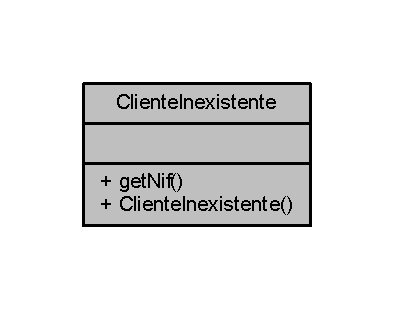
\includegraphics[width=189pt]{class_cliente_inexistente__coll__graph}
\end{center}
\end{figure}
\subsection*{Membros públicos}
\begin{DoxyCompactItemize}
\item 
\hypertarget{class_cliente_inexistente_a020a5414aa9e2714ddeb952a6fd450f4}{}int {\bfseries get\+Nif} ()\label{class_cliente_inexistente_a020a5414aa9e2714ddeb952a6fd450f4}

\item 
\hypertarget{class_cliente_inexistente_a631838af9356603343f06a3492dc20ee}{}{\bfseries Cliente\+Inexistente} (int nif)\label{class_cliente_inexistente_a631838af9356603343f06a3492dc20ee}

\end{DoxyCompactItemize}


A documentação para esta classe foi gerada a partir do seguinte ficheiro\+:\begin{DoxyCompactItemize}
\item 
C\+:/\+Users/josea/\+Documents/\+Git\+Hub/\+A\+E\+D\+A-\/\+Part1/Cliente.\+h\end{DoxyCompactItemize}

\hypertarget{class_empresa}{}\section{Referência à classe Empresa}
\label{class_empresa}\index{Empresa@{Empresa}}


Diagrama de colaboração para Empresa\+:
\nopagebreak
\begin{figure}[H]
\begin{center}
\leavevmode
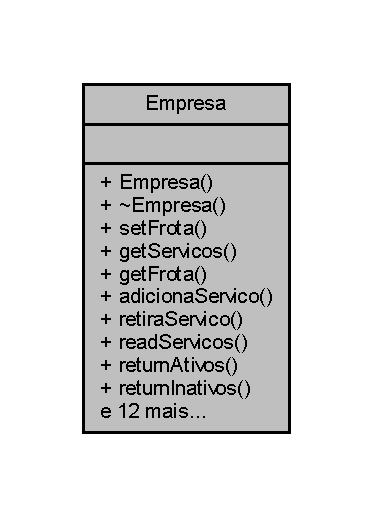
\includegraphics[width=179pt]{class_empresa__coll__graph}
\end{center}
\end{figure}
\subsection*{Membros públicos}
\begin{DoxyCompactItemize}
\item 
\hyperlink{class_empresa_ac5bccaf3758b25fea4803a63d4362236}{Empresa} (string nome)
\begin{DoxyCompactList}\small\item\em Cria uma \hyperlink{class_empresa}{Empresa} usando os parâmetros para definir as sua caracteristicas. \end{DoxyCompactList}\item 
void \hyperlink{class_empresa_a30c9127acfb46b0617749fd9c3151b22}{set\+Frota} (\hyperlink{class_frota}{Frota} frota)
\begin{DoxyCompactList}\small\item\em Atribui um frota a uma \hyperlink{class_empresa}{Empresa}. \end{DoxyCompactList}\item 
vector$<$ \hyperlink{class_servico}{Servico} $\ast$ $>$ \hyperlink{class_empresa_a5b64141cd1395ed4ba4b12822986ec98}{get\+Servicos} () const 
\begin{DoxyCompactList}\small\item\em Obtém o vetor que guarda todos os Serviços da \hyperlink{class_empresa}{Empresa}. \end{DoxyCompactList}\item 
\hyperlink{class_frota}{Frota} \hyperlink{class_empresa_afd239717a3e8e57b28e722df306941ce}{get\+Frota} () const 
\begin{DoxyCompactList}\small\item\em Obtém a frota da empresa. \end{DoxyCompactList}\item 
void \hyperlink{class_empresa_a3e6883a21a837c02cdaae73b401b75d7}{adiciona\+Servico} (\hyperlink{class_servico}{Servico} $\ast$s1)
\begin{DoxyCompactList}\small\item\em Adiciona um Serviço ao vetor. \end{DoxyCompactList}\item 
void \hyperlink{class_empresa_a17e3b2a202233623f8c9dc183b65364e}{retira\+Servico} (\hyperlink{class_servico}{Servico} $\ast$s1)
\begin{DoxyCompactList}\small\item\em Retira um Serviço do vetor, caso este lá esteja, caso contrário lança a excessão \hyperlink{class_cliente_inexistente}{Cliente\+Inexistente}. \end{DoxyCompactList}\item 
void \hyperlink{class_empresa_abf38596df14beba52315687b699fe087}{read\+Servicos} () const 
\begin{DoxyCompactList}\small\item\em Lê todas as informações dos serviços e dos clientes que usufruem deles. \end{DoxyCompactList}\item 
vector$<$ \hyperlink{class_servico}{Servico} $\ast$ $>$ \hyperlink{class_empresa_a94550ff669545ff0cd03f85118a63394}{return\+Ativos} ()
\begin{DoxyCompactList}\small\item\em Cria um vetor com todos os serviços ativos. \end{DoxyCompactList}\item 
vector$<$ \hyperlink{class_servico}{Servico} $\ast$ $>$ \hyperlink{class_empresa_ae03b8956798a193ea9140394f744b863}{return\+Inativos} ()
\begin{DoxyCompactList}\small\item\em Cria um vetor com todos os serviços inativos. \end{DoxyCompactList}\item 
void \hyperlink{class_empresa_a29c441849b5df54979d39f5e0c7607e2}{print\+Servicos} ()
\begin{DoxyCompactList}\small\item\em Imprime todas as informações dos serviços do vetor. \end{DoxyCompactList}\item 
vector$<$ \hyperlink{class_servico}{Servico} $\ast$ $>$ \hyperlink{class_empresa_aee257392591e04103105366515815b2c}{servico\+Cliente} (string nome, unsigned int nif)
\begin{DoxyCompactList}\small\item\em Cria um vetor com todos os serviços cujo cliente identificado pelos parâmetros. \end{DoxyCompactList}\item 
void \hyperlink{class_empresa_abafc415ff93409f9f0f66ad6e1bade32}{save\+Empresa} ()
\begin{DoxyCompactList}\small\item\em Guarda um \hyperlink{class_empresa}{Empresa}, e consequentemente todas as suas informações, num ficheiro a especificar. \end{DoxyCompactList}\item 
int \hyperlink{class_empresa_a386b43304a0482047274f95b3442f9ff}{load\+Empresa} ()
\begin{DoxyCompactList}\small\item\em Carrega uma \hyperlink{class_empresa}{Empresa} criada e guardada previamente num ficheiro a especificar. \end{DoxyCompactList}\item 
\hypertarget{class_empresa_a4514b68f6549fa2860e74e788a74a041}{}float {\bfseries get\+Custo\+Cap} () const \label{class_empresa_a4514b68f6549fa2860e74e788a74a041}

\item 
float \hyperlink{class_empresa_ad13572d5f1cd219eac3c5a67ed0cd77f}{get\+Custo\+Cong} () const 
\begin{DoxyCompactList}\small\item\em Obtém o custo extra da capacidade de congelação dos camiões da empresa. \end{DoxyCompactList}\item 
float \hyperlink{class_empresa_a5c0286d07ea42c5d818f8b18aa530d06}{get\+Custo\+Perig} () const 
\begin{DoxyCompactList}\small\item\em Obtém o custo extra da capacidade de transporte de cargas perigosas. \end{DoxyCompactList}\item 
float \hyperlink{class_empresa_a5fff95aab4d58e80e739de0baa473245}{get\+Custo\+Dist} () const 
\begin{DoxyCompactList}\small\item\em Obtém a taxa cobrada por cada km percorrido por um camião da empresa. \end{DoxyCompactList}\item 
\hypertarget{class_empresa_a8f6ad48850f190224c912824fc760aed}{}void {\bfseries set\+Custo\+Cap} (float n)\label{class_empresa_a8f6ad48850f190224c912824fc760aed}

\item 
void \hyperlink{class_empresa_a5e83a7a3a3a19b597c2bd17f16ec0bbb}{set\+Custo\+Cong} (float n)
\begin{DoxyCompactList}\small\item\em Altera o custo extra de um camião com capacidade de congelação. \end{DoxyCompactList}\item 
void \hyperlink{class_empresa_a8a467aca65f03f7dcf4b745923567f7d}{set\+Custo\+Perig} (float n)
\begin{DoxyCompactList}\small\item\em Altera o custo extra de um camião com capacidade de transportar cargas perigosas. \end{DoxyCompactList}\item 
void \hyperlink{class_empresa_abe767c7e1ce6e087197e1c215585613c}{set\+Custo\+Dist} (float n)
\begin{DoxyCompactList}\small\item\em Altera a taxa cobrada por cada quilómetro percorrido pelos camiões da empresa. \end{DoxyCompactList}\end{DoxyCompactItemize}


\subsection{Documentação dos Construtores \& Destrutor}
\hypertarget{class_empresa_ac5bccaf3758b25fea4803a63d4362236}{}\index{Empresa@{Empresa}!Empresa@{Empresa}}
\index{Empresa@{Empresa}!Empresa@{Empresa}}
\subsubsection[{Empresa(string nome)}]{\setlength{\rightskip}{0pt plus 5cm}Empresa\+::\+Empresa (
\begin{DoxyParamCaption}
\item[{string}]{nome}
\end{DoxyParamCaption}
)}\label{class_empresa_ac5bccaf3758b25fea4803a63d4362236}


Cria uma \hyperlink{class_empresa}{Empresa} usando os parâmetros para definir as sua caracteristicas. 


\begin{DoxyParams}{Parâmetros}
{\em nome} & Nome da \hyperlink{class_empresa}{Empresa} \\
\hline
\end{DoxyParams}
\begin{DoxyReturn}{Retorna}
Esta função não possui retorno 
\end{DoxyReturn}


\subsection{Documentação dos métodos}
\hypertarget{class_empresa_a3e6883a21a837c02cdaae73b401b75d7}{}\index{Empresa@{Empresa}!adiciona\+Servico@{adiciona\+Servico}}
\index{adiciona\+Servico@{adiciona\+Servico}!Empresa@{Empresa}}
\subsubsection[{adiciona\+Servico(\+Servico $\ast$s1)}]{\setlength{\rightskip}{0pt plus 5cm}void Empresa\+::adiciona\+Servico (
\begin{DoxyParamCaption}
\item[{{\bf Servico} $\ast$}]{s1}
\end{DoxyParamCaption}
)}\label{class_empresa_a3e6883a21a837c02cdaae73b401b75d7}


Adiciona um Serviço ao vetor. 


\begin{DoxyParams}{Parâmetros}
{\em s1} & Serviço a adicionar \\
\hline
\end{DoxyParams}
\begin{DoxyReturn}{Retorna}
Esta função não possui retorno 
\end{DoxyReturn}
\hypertarget{class_empresa_ad13572d5f1cd219eac3c5a67ed0cd77f}{}\index{Empresa@{Empresa}!get\+Custo\+Cong@{get\+Custo\+Cong}}
\index{get\+Custo\+Cong@{get\+Custo\+Cong}!Empresa@{Empresa}}
\subsubsection[{get\+Custo\+Cong() const }]{\setlength{\rightskip}{0pt plus 5cm}float Empresa\+::get\+Custo\+Cong (
\begin{DoxyParamCaption}
{}
\end{DoxyParamCaption}
) const}\label{class_empresa_ad13572d5f1cd219eac3c5a67ed0cd77f}


Obtém o custo extra da capacidade de congelação dos camiões da empresa. 

\begin{DoxyReturn}{Retorna}
Retorna o custo extra da capacidade de congelação de camiões desta empresa 
\end{DoxyReturn}
\hypertarget{class_empresa_a5fff95aab4d58e80e739de0baa473245}{}\index{Empresa@{Empresa}!get\+Custo\+Dist@{get\+Custo\+Dist}}
\index{get\+Custo\+Dist@{get\+Custo\+Dist}!Empresa@{Empresa}}
\subsubsection[{get\+Custo\+Dist() const }]{\setlength{\rightskip}{0pt plus 5cm}float Empresa\+::get\+Custo\+Dist (
\begin{DoxyParamCaption}
{}
\end{DoxyParamCaption}
) const}\label{class_empresa_a5fff95aab4d58e80e739de0baa473245}


Obtém a taxa cobrada por cada km percorrido por um camião da empresa. 

\begin{DoxyReturn}{Retorna}
Retorna o valor da taxa em €/km 
\end{DoxyReturn}
\hypertarget{class_empresa_a5c0286d07ea42c5d818f8b18aa530d06}{}\index{Empresa@{Empresa}!get\+Custo\+Perig@{get\+Custo\+Perig}}
\index{get\+Custo\+Perig@{get\+Custo\+Perig}!Empresa@{Empresa}}
\subsubsection[{get\+Custo\+Perig() const }]{\setlength{\rightskip}{0pt plus 5cm}float Empresa\+::get\+Custo\+Perig (
\begin{DoxyParamCaption}
{}
\end{DoxyParamCaption}
) const}\label{class_empresa_a5c0286d07ea42c5d818f8b18aa530d06}


Obtém o custo extra da capacidade de transporte de cargas perigosas. 

\begin{DoxyReturn}{Retorna}
Retorna o custo extra da capacidade de transporte de cargas perigosasde camiões desta empresa 
\end{DoxyReturn}
\hypertarget{class_empresa_afd239717a3e8e57b28e722df306941ce}{}\index{Empresa@{Empresa}!get\+Frota@{get\+Frota}}
\index{get\+Frota@{get\+Frota}!Empresa@{Empresa}}
\subsubsection[{get\+Frota() const }]{\setlength{\rightskip}{0pt plus 5cm}{\bf Frota} Empresa\+::get\+Frota (
\begin{DoxyParamCaption}
{}
\end{DoxyParamCaption}
) const}\label{class_empresa_afd239717a3e8e57b28e722df306941ce}


Obtém a frota da empresa. 

\begin{DoxyReturn}{Retorna}
Retorna o objeto \hyperlink{class_frota}{Frota} com a frota da empresa 
\end{DoxyReturn}
\hypertarget{class_empresa_a5b64141cd1395ed4ba4b12822986ec98}{}\index{Empresa@{Empresa}!get\+Servicos@{get\+Servicos}}
\index{get\+Servicos@{get\+Servicos}!Empresa@{Empresa}}
\subsubsection[{get\+Servicos() const }]{\setlength{\rightskip}{0pt plus 5cm}vector$<$ {\bf Servico} $\ast$ $>$ Empresa\+::get\+Servicos (
\begin{DoxyParamCaption}
{}
\end{DoxyParamCaption}
) const}\label{class_empresa_a5b64141cd1395ed4ba4b12822986ec98}


Obtém o vetor que guarda todos os Serviços da \hyperlink{class_empresa}{Empresa}. 

\begin{DoxyReturn}{Retorna}
Retorna o vetor 
\end{DoxyReturn}
\hypertarget{class_empresa_a386b43304a0482047274f95b3442f9ff}{}\index{Empresa@{Empresa}!load\+Empresa@{load\+Empresa}}
\index{load\+Empresa@{load\+Empresa}!Empresa@{Empresa}}
\subsubsection[{load\+Empresa()}]{\setlength{\rightskip}{0pt plus 5cm}int Empresa\+::load\+Empresa (
\begin{DoxyParamCaption}
{}
\end{DoxyParamCaption}
)}\label{class_empresa_a386b43304a0482047274f95b3442f9ff}


Carrega uma \hyperlink{class_empresa}{Empresa} criada e guardada previamente num ficheiro a especificar. 

\begin{DoxyReturn}{Retorna}
Retorna 0; 
\end{DoxyReturn}
\hypertarget{class_empresa_a29c441849b5df54979d39f5e0c7607e2}{}\index{Empresa@{Empresa}!print\+Servicos@{print\+Servicos}}
\index{print\+Servicos@{print\+Servicos}!Empresa@{Empresa}}
\subsubsection[{print\+Servicos()}]{\setlength{\rightskip}{0pt plus 5cm}void Empresa\+::print\+Servicos (
\begin{DoxyParamCaption}
{}
\end{DoxyParamCaption}
)}\label{class_empresa_a29c441849b5df54979d39f5e0c7607e2}


Imprime todas as informações dos serviços do vetor. 

\begin{DoxyReturn}{Retorna}
Esta função não possui retorno 
\end{DoxyReturn}
\hypertarget{class_empresa_abf38596df14beba52315687b699fe087}{}\index{Empresa@{Empresa}!read\+Servicos@{read\+Servicos}}
\index{read\+Servicos@{read\+Servicos}!Empresa@{Empresa}}
\subsubsection[{read\+Servicos() const }]{\setlength{\rightskip}{0pt plus 5cm}void Empresa\+::read\+Servicos (
\begin{DoxyParamCaption}
{}
\end{DoxyParamCaption}
) const}\label{class_empresa_abf38596df14beba52315687b699fe087}


Lê todas as informações dos serviços e dos clientes que usufruem deles. 

\begin{DoxyReturn}{Retorna}
Esta função não possui retorno 
\end{DoxyReturn}
\hypertarget{class_empresa_a17e3b2a202233623f8c9dc183b65364e}{}\index{Empresa@{Empresa}!retira\+Servico@{retira\+Servico}}
\index{retira\+Servico@{retira\+Servico}!Empresa@{Empresa}}
\subsubsection[{retira\+Servico(\+Servico $\ast$s1)}]{\setlength{\rightskip}{0pt plus 5cm}void Empresa\+::retira\+Servico (
\begin{DoxyParamCaption}
\item[{{\bf Servico} $\ast$}]{s1}
\end{DoxyParamCaption}
)}\label{class_empresa_a17e3b2a202233623f8c9dc183b65364e}


Retira um Serviço do vetor, caso este lá esteja, caso contrário lança a excessão \hyperlink{class_cliente_inexistente}{Cliente\+Inexistente}. 


\begin{DoxyParams}{Parâmetros}
{\em s1} & Serviço a retirar \\
\hline
\end{DoxyParams}
\begin{DoxyReturn}{Retorna}
Esta função não possui retorno 
\end{DoxyReturn}
\hypertarget{class_empresa_a94550ff669545ff0cd03f85118a63394}{}\index{Empresa@{Empresa}!return\+Ativos@{return\+Ativos}}
\index{return\+Ativos@{return\+Ativos}!Empresa@{Empresa}}
\subsubsection[{return\+Ativos()}]{\setlength{\rightskip}{0pt plus 5cm}vector$<$ {\bf Servico} $\ast$ $>$ Empresa\+::return\+Ativos (
\begin{DoxyParamCaption}
{}
\end{DoxyParamCaption}
)}\label{class_empresa_a94550ff669545ff0cd03f85118a63394}


Cria um vetor com todos os serviços ativos. 

\begin{DoxyReturn}{Retorna}
Retorna o vetor 
\end{DoxyReturn}
\hypertarget{class_empresa_ae03b8956798a193ea9140394f744b863}{}\index{Empresa@{Empresa}!return\+Inativos@{return\+Inativos}}
\index{return\+Inativos@{return\+Inativos}!Empresa@{Empresa}}
\subsubsection[{return\+Inativos()}]{\setlength{\rightskip}{0pt plus 5cm}vector$<$ {\bf Servico} $\ast$ $>$ Empresa\+::return\+Inativos (
\begin{DoxyParamCaption}
{}
\end{DoxyParamCaption}
)}\label{class_empresa_ae03b8956798a193ea9140394f744b863}


Cria um vetor com todos os serviços inativos. 

\begin{DoxyReturn}{Retorna}
Retorna o vetor 
\end{DoxyReturn}
\hypertarget{class_empresa_abafc415ff93409f9f0f66ad6e1bade32}{}\index{Empresa@{Empresa}!save\+Empresa@{save\+Empresa}}
\index{save\+Empresa@{save\+Empresa}!Empresa@{Empresa}}
\subsubsection[{save\+Empresa()}]{\setlength{\rightskip}{0pt plus 5cm}void Empresa\+::save\+Empresa (
\begin{DoxyParamCaption}
{}
\end{DoxyParamCaption}
)}\label{class_empresa_abafc415ff93409f9f0f66ad6e1bade32}


Guarda um \hyperlink{class_empresa}{Empresa}, e consequentemente todas as suas informações, num ficheiro a especificar. 

\begin{DoxyReturn}{Retorna}
Esta função não possui retorno 
\end{DoxyReturn}
\hypertarget{class_empresa_aee257392591e04103105366515815b2c}{}\index{Empresa@{Empresa}!servico\+Cliente@{servico\+Cliente}}
\index{servico\+Cliente@{servico\+Cliente}!Empresa@{Empresa}}
\subsubsection[{servico\+Cliente(string nome, unsigned int nif)}]{\setlength{\rightskip}{0pt plus 5cm}vector$<$ {\bf Servico} $\ast$ $>$ Empresa\+::servico\+Cliente (
\begin{DoxyParamCaption}
\item[{string}]{nome, }
\item[{unsigned int}]{nif}
\end{DoxyParamCaption}
)}\label{class_empresa_aee257392591e04103105366515815b2c}


Cria um vetor com todos os serviços cujo cliente identificado pelos parâmetros. 


\begin{DoxyParams}{Parâmetros}
{\em nome} & Nome do \hyperlink{class_cliente}{Cliente} a pesquisar \\
\hline
{\em nif} & N\+I\+F do \hyperlink{class_cliente}{Cliente} a pesquisar \\
\hline
\end{DoxyParams}
\begin{DoxyReturn}{Retorna}
Retorna o vetor criado 
\end{DoxyReturn}
\hypertarget{class_empresa_a5e83a7a3a3a19b597c2bd17f16ec0bbb}{}\index{Empresa@{Empresa}!set\+Custo\+Cong@{set\+Custo\+Cong}}
\index{set\+Custo\+Cong@{set\+Custo\+Cong}!Empresa@{Empresa}}
\subsubsection[{set\+Custo\+Cong(float n)}]{\setlength{\rightskip}{0pt plus 5cm}void Empresa\+::set\+Custo\+Cong (
\begin{DoxyParamCaption}
\item[{float}]{n}
\end{DoxyParamCaption}
)}\label{class_empresa_a5e83a7a3a3a19b597c2bd17f16ec0bbb}


Altera o custo extra de um camião com capacidade de congelação. 


\begin{DoxyParams}{Parâmetros}
{\em n} & Novo preço \\
\hline
\end{DoxyParams}
\begin{DoxyReturn}{Retorna}
Esta função não poussui retorno 
\end{DoxyReturn}
\hypertarget{class_empresa_abe767c7e1ce6e087197e1c215585613c}{}\index{Empresa@{Empresa}!set\+Custo\+Dist@{set\+Custo\+Dist}}
\index{set\+Custo\+Dist@{set\+Custo\+Dist}!Empresa@{Empresa}}
\subsubsection[{set\+Custo\+Dist(float n)}]{\setlength{\rightskip}{0pt plus 5cm}void Empresa\+::set\+Custo\+Dist (
\begin{DoxyParamCaption}
\item[{float}]{n}
\end{DoxyParamCaption}
)}\label{class_empresa_abe767c7e1ce6e087197e1c215585613c}


Altera a taxa cobrada por cada quilómetro percorrido pelos camiões da empresa. 


\begin{DoxyParams}{Parâmetros}
{\em n} & Nova taxa \\
\hline
\end{DoxyParams}
\begin{DoxyReturn}{Retorna}
Esta função não poussui retorno 
\end{DoxyReturn}
\hypertarget{class_empresa_a8a467aca65f03f7dcf4b745923567f7d}{}\index{Empresa@{Empresa}!set\+Custo\+Perig@{set\+Custo\+Perig}}
\index{set\+Custo\+Perig@{set\+Custo\+Perig}!Empresa@{Empresa}}
\subsubsection[{set\+Custo\+Perig(float n)}]{\setlength{\rightskip}{0pt plus 5cm}void Empresa\+::set\+Custo\+Perig (
\begin{DoxyParamCaption}
\item[{float}]{n}
\end{DoxyParamCaption}
)}\label{class_empresa_a8a467aca65f03f7dcf4b745923567f7d}


Altera o custo extra de um camião com capacidade de transportar cargas perigosas. 


\begin{DoxyParams}{Parâmetros}
{\em n} & Novo preço \\
\hline
\end{DoxyParams}
\begin{DoxyReturn}{Retorna}
Esta função não poussui retorno 
\end{DoxyReturn}
\hypertarget{class_empresa_a30c9127acfb46b0617749fd9c3151b22}{}\index{Empresa@{Empresa}!set\+Frota@{set\+Frota}}
\index{set\+Frota@{set\+Frota}!Empresa@{Empresa}}
\subsubsection[{set\+Frota(\+Frota frota)}]{\setlength{\rightskip}{0pt plus 5cm}void Empresa\+::set\+Frota (
\begin{DoxyParamCaption}
\item[{{\bf Frota}}]{frota}
\end{DoxyParamCaption}
)}\label{class_empresa_a30c9127acfb46b0617749fd9c3151b22}


Atribui um frota a uma \hyperlink{class_empresa}{Empresa}. 


\begin{DoxyParams}{Parâmetros}
{\em frota} & \hyperlink{class_frota}{Frota} a atribuir \\
\hline
\end{DoxyParams}
\begin{DoxyReturn}{Retorna}
Esta função não possui retorno 
\end{DoxyReturn}


A documentação para esta classe foi gerada a partir dos seguintes ficheiros\+:\begin{DoxyCompactItemize}
\item 
C\+:/\+Users/josea/\+Documents/\+Git\+Hub/\+A\+E\+D\+A-\/\+Part1/Empresa.\+h\item 
C\+:/\+Users/josea/\+Documents/\+Git\+Hub/\+A\+E\+D\+A-\/\+Part1/Empresa.\+cpp\end{DoxyCompactItemize}

\hypertarget{class_frota}{}\section{Referência à classe Frota}
\label{class_frota}\index{Frota@{Frota}}


Diagrama de colaboração para Frota\+:
\nopagebreak
\begin{figure}[H]
\begin{center}
\leavevmode
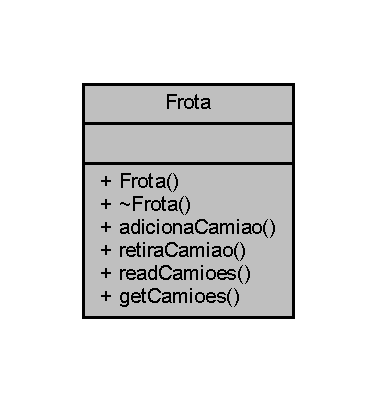
\includegraphics[width=181pt]{class_frota__coll__graph}
\end{center}
\end{figure}
\subsection*{Membros públicos}
\begin{DoxyCompactItemize}
\item 
\hyperlink{class_frota_a0c7df66d110f59687c6c0b4a389be3a5}{Frota} ()
\begin{DoxyCompactList}\small\item\em Cria uma \hyperlink{class_frota}{Frota} sem parâmetros. \end{DoxyCompactList}\item 
void \hyperlink{class_frota_acaee94330b568acfac215c948b14bbce}{adiciona\+Camiao} (\hyperlink{class_camiao}{Camiao} $\ast$c1)
\begin{DoxyCompactList}\small\item\em Adiciona um Camião à frota. \end{DoxyCompactList}\item 
void \hyperlink{class_frota_a1c41f85e1a72c187cfd42308e97e187b}{retira\+Camiao} (\hyperlink{class_camiao}{Camiao} $\ast$c1)
\begin{DoxyCompactList}\small\item\em Retira um Camião da frota, caso este lá esteja, caso contrário lança a excessão \hyperlink{class_camiao_inexistente}{Camiao\+Inexistente}. \end{DoxyCompactList}\item 
void \hyperlink{class_frota_a500d79d6e1e93e12311ad3a6070a9930}{read\+Camioes} () const 
\begin{DoxyCompactList}\small\item\em Imprime todas as informações dos camiões da frota. \end{DoxyCompactList}\item 
vector$<$ \hyperlink{class_camiao}{Camiao} $\ast$ $>$ \hyperlink{class_frota_a16889ffed14ba42e65d5f4e1fdf0887d}{get\+Camioes} ()
\begin{DoxyCompactList}\small\item\em Obtém o vetor que guarda todos os camiões da frota. \end{DoxyCompactList}\end{DoxyCompactItemize}


\subsection{Documentação dos Construtores \& Destrutor}
\hypertarget{class_frota_a0c7df66d110f59687c6c0b4a389be3a5}{}\index{Frota@{Frota}!Frota@{Frota}}
\index{Frota@{Frota}!Frota@{Frota}}
\subsubsection[{Frota()}]{\setlength{\rightskip}{0pt plus 5cm}Frota\+::\+Frota (
\begin{DoxyParamCaption}
{}
\end{DoxyParamCaption}
)}\label{class_frota_a0c7df66d110f59687c6c0b4a389be3a5}


Cria uma \hyperlink{class_frota}{Frota} sem parâmetros. 

\begin{DoxyReturn}{Retorna}
Esta função não possui retorno 
\end{DoxyReturn}


\subsection{Documentação dos métodos}
\hypertarget{class_frota_acaee94330b568acfac215c948b14bbce}{}\index{Frota@{Frota}!adiciona\+Camiao@{adiciona\+Camiao}}
\index{adiciona\+Camiao@{adiciona\+Camiao}!Frota@{Frota}}
\subsubsection[{adiciona\+Camiao(\+Camiao $\ast$c1)}]{\setlength{\rightskip}{0pt plus 5cm}void Frota\+::adiciona\+Camiao (
\begin{DoxyParamCaption}
\item[{{\bf Camiao} $\ast$}]{c1}
\end{DoxyParamCaption}
)}\label{class_frota_acaee94330b568acfac215c948b14bbce}


Adiciona um Camião à frota. 


\begin{DoxyParams}{Parâmetros}
{\em c1} & Camião a adicionar \\
\hline
\end{DoxyParams}
\begin{DoxyReturn}{Retorna}
Esta função não possui retorno 
\end{DoxyReturn}
\hypertarget{class_frota_a16889ffed14ba42e65d5f4e1fdf0887d}{}\index{Frota@{Frota}!get\+Camioes@{get\+Camioes}}
\index{get\+Camioes@{get\+Camioes}!Frota@{Frota}}
\subsubsection[{get\+Camioes()}]{\setlength{\rightskip}{0pt plus 5cm}vector$<$ {\bf Camiao} $\ast$ $>$ Frota\+::get\+Camioes (
\begin{DoxyParamCaption}
{}
\end{DoxyParamCaption}
)}\label{class_frota_a16889ffed14ba42e65d5f4e1fdf0887d}


Obtém o vetor que guarda todos os camiões da frota. 

\begin{DoxyReturn}{Retorna}
Retorna o vetor 
\end{DoxyReturn}
\hypertarget{class_frota_a500d79d6e1e93e12311ad3a6070a9930}{}\index{Frota@{Frota}!read\+Camioes@{read\+Camioes}}
\index{read\+Camioes@{read\+Camioes}!Frota@{Frota}}
\subsubsection[{read\+Camioes() const }]{\setlength{\rightskip}{0pt plus 5cm}void Frota\+::read\+Camioes (
\begin{DoxyParamCaption}
{}
\end{DoxyParamCaption}
) const}\label{class_frota_a500d79d6e1e93e12311ad3a6070a9930}


Imprime todas as informações dos camiões da frota. 

\begin{DoxyReturn}{Retorna}
Esta função não possui retorno 
\end{DoxyReturn}
\hypertarget{class_frota_a1c41f85e1a72c187cfd42308e97e187b}{}\index{Frota@{Frota}!retira\+Camiao@{retira\+Camiao}}
\index{retira\+Camiao@{retira\+Camiao}!Frota@{Frota}}
\subsubsection[{retira\+Camiao(\+Camiao $\ast$c1)}]{\setlength{\rightskip}{0pt plus 5cm}void Frota\+::retira\+Camiao (
\begin{DoxyParamCaption}
\item[{{\bf Camiao} $\ast$}]{c1}
\end{DoxyParamCaption}
)}\label{class_frota_a1c41f85e1a72c187cfd42308e97e187b}


Retira um Camião da frota, caso este lá esteja, caso contrário lança a excessão \hyperlink{class_camiao_inexistente}{Camiao\+Inexistente}. 


\begin{DoxyParams}{Parâmetros}
{\em c1} & Camião a retirar \\
\hline
\end{DoxyParams}
\begin{DoxyReturn}{Retorna}
Esta função não possui retorno 
\end{DoxyReturn}


A documentação para esta classe foi gerada a partir dos seguintes ficheiros\+:\begin{DoxyCompactItemize}
\item 
C\+:/\+Users/josea/\+Documents/\+Git\+Hub/\+A\+E\+D\+A-\/\+Part1/Frota.\+h\item 
C\+:/\+Users/josea/\+Documents/\+Git\+Hub/\+A\+E\+D\+A-\/\+Part1/Frota.\+cpp\end{DoxyCompactItemize}

\hypertarget{class_servico}{}\section{Referência à classe Servico}
\label{class_servico}\index{Servico@{Servico}}


Diagrama de colaboração para Servico\+:
\nopagebreak
\begin{figure}[H]
\begin{center}
\leavevmode
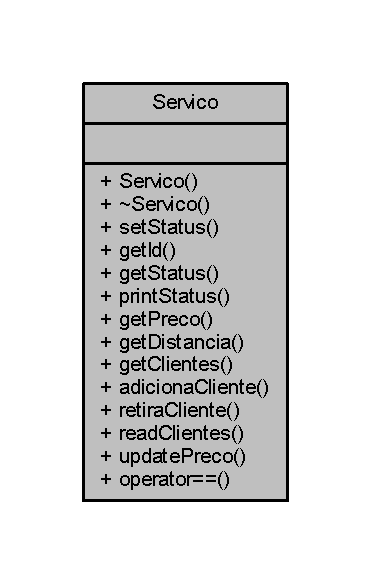
\includegraphics[width=178pt]{class_servico__coll__graph}
\end{center}
\end{figure}
\subsection*{Membros públicos}
\begin{DoxyCompactItemize}
\item 
\hyperlink{class_servico_ad6f73e597087d194f6a768f5b49174a4}{Servico} (int id, float preco, float distancia)
\begin{DoxyCompactList}\small\item\em Cria um Serviço usando os parâmetros para definir as sua caracteristicas. \end{DoxyCompactList}\item 
void \hyperlink{class_servico_a9a12bcdd4adb4dcb9718f6ccc4320e2e}{set\+Status} (bool status)
\begin{DoxyCompactList}\small\item\em Atribui um status a um Serviço, ativo(true) ou inativo(false) \end{DoxyCompactList}\item 
int \hyperlink{class_servico_aeedaf81332746435112616620626f8a0}{get\+Id} () const 
\begin{DoxyCompactList}\small\item\em Obtém o I\+D de um Serviço. \end{DoxyCompactList}\item 
bool \hyperlink{class_servico_ac4da7c7738bc5d0a186676ed72eb3f7f}{get\+Status} () const 
\begin{DoxyCompactList}\small\item\em Verifica se um Serviço está ou não ativo. \end{DoxyCompactList}\item 
string \hyperlink{class_servico_aca8339e45a5072b69f538d9a6791084e}{print\+Status} ()
\begin{DoxyCompactList}\small\item\em Averigua o valor lógico do status. \end{DoxyCompactList}\item 
float \hyperlink{class_servico_a7eea58bc4405f61335bddf3fc25bfafa}{get\+Preco} () const 
\begin{DoxyCompactList}\small\item\em Obtém o Preço de um Serviço. \end{DoxyCompactList}\item 
float \hyperlink{class_servico_a07f492f6984fa33781adbedafe3d7977}{get\+Distancia} () const 
\begin{DoxyCompactList}\small\item\em Obtém a distância necessária para executar o serviço. \end{DoxyCompactList}\item 
vector$<$ \hyperlink{class_cliente}{Cliente} $\ast$ $>$ \hyperlink{class_servico_a3e6faedd16eb2027986b032c1fe601ce}{get\+Clientes} () const 
\begin{DoxyCompactList}\small\item\em Obtém o vetor que guarda todos os Clientes. \end{DoxyCompactList}\item 
void \hyperlink{class_servico_a230392fbbe40d5d4cb5198f65ba26cd5}{adiciona\+Cliente} (\hyperlink{class_cliente}{Cliente} $\ast$j1)
\begin{DoxyCompactList}\small\item\em Adiciona um \hyperlink{class_cliente}{Cliente} ao vetor. \end{DoxyCompactList}\item 
void \hyperlink{class_servico_ab6fedbc606ac14cd7181be469d763e91}{retira\+Cliente} (\hyperlink{class_cliente}{Cliente} $\ast$j1)
\begin{DoxyCompactList}\small\item\em Retira um \hyperlink{class_cliente}{Cliente} do vetor, caso este lá esteja, caso contrário lança a excessão \hyperlink{class_cliente_inexistente}{Cliente\+Inexistente}. \end{DoxyCompactList}\item 
void \hyperlink{class_servico_a98156d44790f7aa46e9af802a5c54f2d}{read\+Clientes} () const 
\begin{DoxyCompactList}\small\item\em Imprime todas as informações dos clientes do vetor. \end{DoxyCompactList}\item 
void \hyperlink{class_servico_a596e378b994c4033d12e180129316f4b}{update\+Preco} (float preco)
\begin{DoxyCompactList}\small\item\em Altera, se necessário, o preço de um Serviço. \end{DoxyCompactList}\item 
bool \hyperlink{class_servico_a3b5df4e06c2e553584762c9047fc470f}{operator==} (const \hyperlink{class_servico}{Servico} \&s1)
\begin{DoxyCompactList}\small\item\em Operador utilizado para verificar se dois serviços são iguais. \end{DoxyCompactList}\end{DoxyCompactItemize}


\subsection{Documentação dos Construtores \& Destrutor}
\hypertarget{class_servico_ad6f73e597087d194f6a768f5b49174a4}{}\index{Servico@{Servico}!Servico@{Servico}}
\index{Servico@{Servico}!Servico@{Servico}}
\subsubsection[{Servico(int id, float preco, float distancia)}]{\setlength{\rightskip}{0pt plus 5cm}Servico\+::\+Servico (
\begin{DoxyParamCaption}
\item[{int}]{id, }
\item[{float}]{preco, }
\item[{float}]{distancia}
\end{DoxyParamCaption}
)}\label{class_servico_ad6f73e597087d194f6a768f5b49174a4}


Cria um Serviço usando os parâmetros para definir as sua caracteristicas. 


\begin{DoxyParams}{Parâmetros}
{\em id} & I\+D do Serviço \\
\hline
{\em preco} & Preço do Serviço em custo por quilograma de carga (€/kg) \\
\hline
{\em distancia} & Distância que o camião vai percorrer durante o serviço (km) \\
\hline
\end{DoxyParams}
\begin{DoxyReturn}{Retorna}
Esta função não possui retorno 
\end{DoxyReturn}


\subsection{Documentação dos métodos}
\hypertarget{class_servico_a230392fbbe40d5d4cb5198f65ba26cd5}{}\index{Servico@{Servico}!adiciona\+Cliente@{adiciona\+Cliente}}
\index{adiciona\+Cliente@{adiciona\+Cliente}!Servico@{Servico}}
\subsubsection[{adiciona\+Cliente(\+Cliente $\ast$j1)}]{\setlength{\rightskip}{0pt plus 5cm}void Servico\+::adiciona\+Cliente (
\begin{DoxyParamCaption}
\item[{{\bf Cliente} $\ast$}]{j1}
\end{DoxyParamCaption}
)}\label{class_servico_a230392fbbe40d5d4cb5198f65ba26cd5}


Adiciona um \hyperlink{class_cliente}{Cliente} ao vetor. 


\begin{DoxyParams}{Parâmetros}
{\em j1} & \hyperlink{class_cliente}{Cliente} a adicionar \\
\hline
\end{DoxyParams}
\begin{DoxyReturn}{Retorna}
Esta função não possui retorno 
\end{DoxyReturn}
\hypertarget{class_servico_a3e6faedd16eb2027986b032c1fe601ce}{}\index{Servico@{Servico}!get\+Clientes@{get\+Clientes}}
\index{get\+Clientes@{get\+Clientes}!Servico@{Servico}}
\subsubsection[{get\+Clientes() const }]{\setlength{\rightskip}{0pt plus 5cm}vector$<$ {\bf Cliente} $\ast$ $>$ Servico\+::get\+Clientes (
\begin{DoxyParamCaption}
{}
\end{DoxyParamCaption}
) const}\label{class_servico_a3e6faedd16eb2027986b032c1fe601ce}


Obtém o vetor que guarda todos os Clientes. 

\begin{DoxyReturn}{Retorna}
Retorna o vetor 
\end{DoxyReturn}
\hypertarget{class_servico_a07f492f6984fa33781adbedafe3d7977}{}\index{Servico@{Servico}!get\+Distancia@{get\+Distancia}}
\index{get\+Distancia@{get\+Distancia}!Servico@{Servico}}
\subsubsection[{get\+Distancia() const }]{\setlength{\rightskip}{0pt plus 5cm}float Servico\+::get\+Distancia (
\begin{DoxyParamCaption}
{}
\end{DoxyParamCaption}
) const}\label{class_servico_a07f492f6984fa33781adbedafe3d7977}


Obtém a distância necessária para executar o serviço. 

\begin{DoxyReturn}{Retorna}
Retorna o valor em km 
\end{DoxyReturn}
\hypertarget{class_servico_aeedaf81332746435112616620626f8a0}{}\index{Servico@{Servico}!get\+Id@{get\+Id}}
\index{get\+Id@{get\+Id}!Servico@{Servico}}
\subsubsection[{get\+Id() const }]{\setlength{\rightskip}{0pt plus 5cm}int Servico\+::get\+Id (
\begin{DoxyParamCaption}
{}
\end{DoxyParamCaption}
) const}\label{class_servico_aeedaf81332746435112616620626f8a0}


Obtém o I\+D de um Serviço. 

\begin{DoxyReturn}{Retorna}
Retorna o I\+D de um Serviço 
\end{DoxyReturn}
\hypertarget{class_servico_a7eea58bc4405f61335bddf3fc25bfafa}{}\index{Servico@{Servico}!get\+Preco@{get\+Preco}}
\index{get\+Preco@{get\+Preco}!Servico@{Servico}}
\subsubsection[{get\+Preco() const }]{\setlength{\rightskip}{0pt plus 5cm}float Servico\+::get\+Preco (
\begin{DoxyParamCaption}
{}
\end{DoxyParamCaption}
) const}\label{class_servico_a7eea58bc4405f61335bddf3fc25bfafa}


Obtém o Preço de um Serviço. 

\begin{DoxyReturn}{Retorna}
Retorna o Preço de um Serviço 
\end{DoxyReturn}
\hypertarget{class_servico_ac4da7c7738bc5d0a186676ed72eb3f7f}{}\index{Servico@{Servico}!get\+Status@{get\+Status}}
\index{get\+Status@{get\+Status}!Servico@{Servico}}
\subsubsection[{get\+Status() const }]{\setlength{\rightskip}{0pt plus 5cm}bool Servico\+::get\+Status (
\begin{DoxyParamCaption}
{}
\end{DoxyParamCaption}
) const}\label{class_servico_ac4da7c7738bc5d0a186676ed72eb3f7f}


Verifica se um Serviço está ou não ativo. 

\begin{DoxyReturn}{Retorna}
Retorna o valor lógico do status 
\end{DoxyReturn}
\hypertarget{class_servico_a3b5df4e06c2e553584762c9047fc470f}{}\index{Servico@{Servico}!operator==@{operator==}}
\index{operator==@{operator==}!Servico@{Servico}}
\subsubsection[{operator==(const Servico \&s1)}]{\setlength{\rightskip}{0pt plus 5cm}bool Servico\+::operator== (
\begin{DoxyParamCaption}
\item[{const {\bf Servico} \&}]{s1}
\end{DoxyParamCaption}
)}\label{class_servico_a3b5df4e06c2e553584762c9047fc470f}


Operador utilizado para verificar se dois serviços são iguais. 


\begin{DoxyParams}{Parâmetros}
{\em s1} & Serviço a comparar \\
\hline
\end{DoxyParams}
\begin{DoxyReturn}{Retorna}
Retorna true se os Serviços forem iguais e false se não forem 
\end{DoxyReturn}
\hypertarget{class_servico_aca8339e45a5072b69f538d9a6791084e}{}\index{Servico@{Servico}!print\+Status@{print\+Status}}
\index{print\+Status@{print\+Status}!Servico@{Servico}}
\subsubsection[{print\+Status()}]{\setlength{\rightskip}{0pt plus 5cm}string Servico\+::print\+Status (
\begin{DoxyParamCaption}
{}
\end{DoxyParamCaption}
)}\label{class_servico_aca8339e45a5072b69f538d9a6791084e}


Averigua o valor lógico do status. 

\begin{DoxyReturn}{Retorna}
Retorna o status de um Serviço, ativo ou inativo 
\end{DoxyReturn}
\hypertarget{class_servico_a98156d44790f7aa46e9af802a5c54f2d}{}\index{Servico@{Servico}!read\+Clientes@{read\+Clientes}}
\index{read\+Clientes@{read\+Clientes}!Servico@{Servico}}
\subsubsection[{read\+Clientes() const }]{\setlength{\rightskip}{0pt plus 5cm}void Servico\+::read\+Clientes (
\begin{DoxyParamCaption}
{}
\end{DoxyParamCaption}
) const}\label{class_servico_a98156d44790f7aa46e9af802a5c54f2d}


Imprime todas as informações dos clientes do vetor. 

\begin{DoxyReturn}{Retorna}
Esta função não possui retorno 
\end{DoxyReturn}
\hypertarget{class_servico_ab6fedbc606ac14cd7181be469d763e91}{}\index{Servico@{Servico}!retira\+Cliente@{retira\+Cliente}}
\index{retira\+Cliente@{retira\+Cliente}!Servico@{Servico}}
\subsubsection[{retira\+Cliente(\+Cliente $\ast$j1)}]{\setlength{\rightskip}{0pt plus 5cm}void Servico\+::retira\+Cliente (
\begin{DoxyParamCaption}
\item[{{\bf Cliente} $\ast$}]{j1}
\end{DoxyParamCaption}
)}\label{class_servico_ab6fedbc606ac14cd7181be469d763e91}


Retira um \hyperlink{class_cliente}{Cliente} do vetor, caso este lá esteja, caso contrário lança a excessão \hyperlink{class_cliente_inexistente}{Cliente\+Inexistente}. 


\begin{DoxyParams}{Parâmetros}
{\em j1} & \hyperlink{class_cliente}{Cliente} a retirar \\
\hline
\end{DoxyParams}
\begin{DoxyReturn}{Retorna}
Esta função não possui retorno 
\end{DoxyReturn}
\hypertarget{class_servico_a9a12bcdd4adb4dcb9718f6ccc4320e2e}{}\index{Servico@{Servico}!set\+Status@{set\+Status}}
\index{set\+Status@{set\+Status}!Servico@{Servico}}
\subsubsection[{set\+Status(bool status)}]{\setlength{\rightskip}{0pt plus 5cm}void Servico\+::set\+Status (
\begin{DoxyParamCaption}
\item[{bool}]{status}
\end{DoxyParamCaption}
)}\label{class_servico_a9a12bcdd4adb4dcb9718f6ccc4320e2e}


Atribui um status a um Serviço, ativo(true) ou inativo(false) 


\begin{DoxyParams}{Parâmetros}
{\em status} & Status a atribuir \\
\hline
\end{DoxyParams}
\begin{DoxyReturn}{Retorna}
Esta função não possui retorno 
\end{DoxyReturn}
\hypertarget{class_servico_a596e378b994c4033d12e180129316f4b}{}\index{Servico@{Servico}!update\+Preco@{update\+Preco}}
\index{update\+Preco@{update\+Preco}!Servico@{Servico}}
\subsubsection[{update\+Preco(float preco)}]{\setlength{\rightskip}{0pt plus 5cm}void Servico\+::update\+Preco (
\begin{DoxyParamCaption}
\item[{float}]{preco}
\end{DoxyParamCaption}
)}\label{class_servico_a596e378b994c4033d12e180129316f4b}


Altera, se necessário, o preço de um Serviço. 


\begin{DoxyParams}{Parâmetros}
{\em preco} & Novo valor (em €/kg) do serviço \\
\hline
\end{DoxyParams}
\begin{DoxyReturn}{Retorna}
Esta função não possui retorno 
\end{DoxyReturn}


A documentação para esta classe foi gerada a partir dos seguintes ficheiros\+:\begin{DoxyCompactItemize}
\item 
C\+:/\+Users/josea/\+Documents/\+Git\+Hub/\+A\+E\+D\+A-\/\+Part1/Servico.\+h\item 
C\+:/\+Users/josea/\+Documents/\+Git\+Hub/\+A\+E\+D\+A-\/\+Part1/Servico.\+cpp\end{DoxyCompactItemize}

\hypertarget{class_servico_inexistente}{}\section{Referência à classe Servico\+Inexistente}
\label{class_servico_inexistente}\index{Servico\+Inexistente@{Servico\+Inexistente}}


Diagrama de colaboração para Servico\+Inexistente\+:
\nopagebreak
\begin{figure}[H]
\begin{center}
\leavevmode
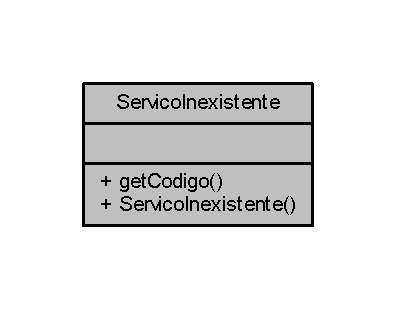
\includegraphics[width=190pt]{class_servico_inexistente__coll__graph}
\end{center}
\end{figure}
\subsection*{Membros públicos}
\begin{DoxyCompactItemize}
\item 
\hypertarget{class_servico_inexistente_a12b2efab8e77afec6604eb4fef14bcf2}{}int {\bfseries get\+Codigo} ()\label{class_servico_inexistente_a12b2efab8e77afec6604eb4fef14bcf2}

\item 
\hypertarget{class_servico_inexistente_a3083bc04a8cd2cdefef0ea04b5ddcb62}{}{\bfseries Servico\+Inexistente} (int codigo)\label{class_servico_inexistente_a3083bc04a8cd2cdefef0ea04b5ddcb62}

\end{DoxyCompactItemize}


A documentação para esta classe foi gerada a partir do seguinte ficheiro\+:\begin{DoxyCompactItemize}
\item 
C\+:/\+Users/josea/\+Documents/\+Git\+Hub/\+A\+E\+D\+A-\/\+Part1/Servico.\+h\end{DoxyCompactItemize}

%--- End generated contents ---

% Index
\backmatter
\newpage
\phantomsection
\clearemptydoublepage
\addcontentsline{toc}{chapter}{Índice}
\printindex

\end{document}
